%----------------------------------------------------------------------------------------
%	PACKAGES AND OTHER DOCUMENT CONFIGURATIONS
%----------------------------------------------------------------------------------------

\documentclass[paper=a4, fontsize=11pt]{scrartcl} % A4 paper and 11pt font size

% ---- Entrada y salida de texto -----

\usepackage[T1]{fontenc} % Use 8-bit encoding that has 256 glyphs
\usepackage[utf8]{inputenc}
%\usepackage{fourier} % Use the Adobe Utopia font for the document - comment this line to return to the LaTeX default

% ---- Idioma --------

\usepackage[spanish, es-tabla]{babel} % Selecciona el español para palabras introducidas automáticamente, p.ej. "septiembre" en la fecha y especifica que se use la palabra Tabla en vez de Cuadro

% ---- Otros paquetes ----
\usepackage{csquotes} %Para permitir el uso de comillas Quotes https://tex.stackexchange.com/questions/36812/isnt-there-any-other-way-of-doing-double-quotes-in-latex-besides
\usepackage[hyphens]{url} % ,href} %para incluir URLs e hipervínculos dentro del texto (aunque hay que instalar href)
\usepackage{hyperref}
\usepackage{color}
\usepackage{graphics,graphicx, floatrow} %para incluir imágenes y notas en las imágenes
\usepackage{graphics,graphicx, float} %para incluir imágenes y colocarlas

\graphicspath {{./img/}}

\usepackage{listings}  %para introducir comandos

\lstdefinestyle{mybash}
{basicstyle=\ttfamily,
  showstringspaces=false,
  commentstyle=\color{red},
  keywordstyle=\color{blue},
  language=bash,
  alsoletter=/,
  basicstyle=\footnotesize,
  numbers=left,
  stepnumber=1,
  showstringspaces=false,
  tabsize=1,
  breaklines=true,
  breakatwhitespace=false,
}
\lstdefinestyle{mysql}
{basicstyle=\ttfamily,
  showstringspaces=false,
  commentstyle=\color{red},
  keywordstyle=\color{blue},
  language=sql,
  basicstyle=\footnotesize,
  numbers=left,
  stepnumber=1,
  showstringspaces=false,
  tabsize=1,
  breaklines=true,
  breakatwhitespace=false,
}


% Para hacer tablas comlejas
%\usepackage{multirow}
%\usepackage{threeparttable}

%\usepackage{sectsty} % Allows customizing section commands
%\allsectionsfont{\centering \normalfont\scshape} % Make all sections centered, the default font and small caps

\usepackage{fancyhdr} % Custom headers and footers
\pagestyle{fancyplain} % Makes all pages in the document conform to the custom headers and footers
\fancyhead{} % No page header - if you want one, create it in the same way as the footers below
\fancyfoot[L]{} % Empty left footer
\fancyfoot[C]{} % Empty center footer
\fancyfoot[R]{\thepage} % Page numbering for right footer
\renewcommand{\headrulewidth}{0pt} % Remove header underlines
\renewcommand{\footrulewidth}{0pt} % Remove footer underlines
\setlength{\headheight}{13.6pt} % Customize the height of the header

\setlength\parindent{0pt} % Removes all indentation from paragraphs - comment this line for an assignment with lots of text

\newcommand{\horrule}[1]{\rule{\linewidth}{#1}} % Create horizontal rule command with 1 argument of height


%----------------------------------------------------------------------------------------
%	TÍTULO Y DATOS DEL ALUMNO
%----------------------------------------------------------------------------------------
\graphicspath{ {img/} }

\title{
\normalfont \normalsize

\includegraphics[width=6cm,height=6cm]{logo}\\
\textsc{\textbf{Bootcamp Especialidad GNU/Linux (2023)}} \\ [25pt] % Your university, school and/or department name(s)
\horrule{0.5pt} \\[0.4cm] % Thin top horizontal rule
\huge Lab 09 - Servicio DNS \\ % The assignment title
\horrule{2pt} \\[0.5cm] % Thick bottom horizontal rule
}


%https://es.overleaf.com/learn/latex/Inserting_Images
%Ruta relativa de   imagenes

\author{Pedro Antonio Mayorgas Parejo} % Nombre y apellidos

\date{\normalsize\today} % Incluye la fecha actual

%----------------------------------------------------------------------------------------
% DOCUMENTO
%----------------------------------------------------------------------------------------

\begin{document}

\maketitle % Muestra el Título

\newpage %inserta un salto de página

\tableofcontents % para generar el índice de contenidos

\newpage

%----------------------------------------------------------------------------------------
%	Cuestión 1
%----------------------------------------------------------------------------------------

\section{Topología de la red}

Debido a la definición del ejercicio, se ha definido la siguiente topología, en la cual están los siguientes dispositivos intermedios:

\begin{itemize}
    \item 2 Switches de Capa 2
    \item 1 DNS autoritativo .net, con capacidad de conexión NAT
    \item 2 Clientes, con nombres registrados en el DNS
\end{itemize}

Esta es la topología de red. Todos los dispositivos tienen la dirección que aparecen o encima o a su izquierda asignada de manera manual.

\begin{figure}[H]
	\centering
	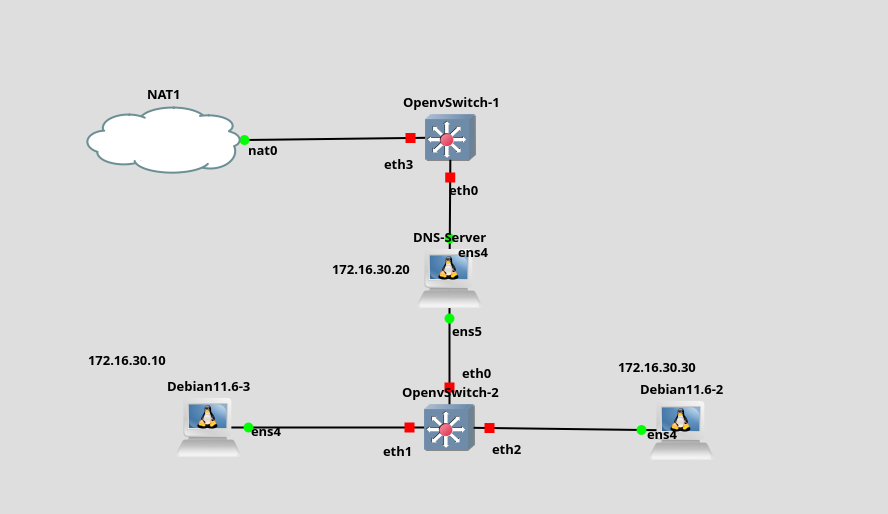
\includegraphics[scale=0.30]{00}
	\caption{Topología de red.}
\end{figure}

\section{Instalación del servicio DNS}

Para la instalación del servicio DNS, tenemos que ejecutar el siguiente comando:

\begin{lstlisting}[style=mybash]
sudo apt install bind9 bind9utils
# FOR DEBUG
sudo apt install dnsutils
\end{lstlisting}

Luego de instalar el servicio DNS, tenemos que configurar el siguiente fichero, para crear una zona y que pueda localizar los ficheros de zona. El fichero en concreto que debemos editar es \textbf{/etc/bind/named.conf}. La línea que añadimos, es una ruta que nos permite indicar las zonas internas que queramos crear para nosotros, es un fichero de configuración adicional de las zonas que gestiona bind9.

\begin{figure}[H]
	\centering
	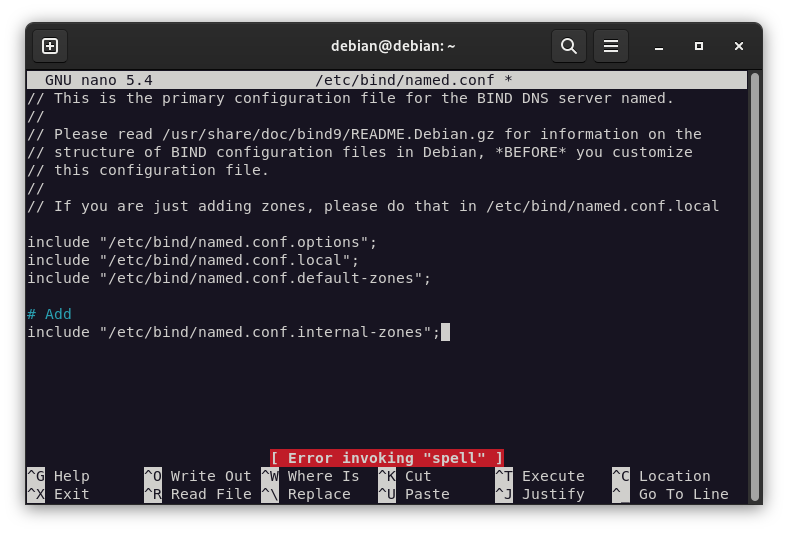
\includegraphics[scale=0.30]{01}
	\caption{Indicando la zona interna.}
\end{figure}

Ahora editamos otro fichero de configuración interna, para permitir un ACL para la red local para que pueda realizar consultas. El fichero en concreto es \textbf{/etc/bind/named.conf.options}.

\begin{figure}[H]
	\centering
	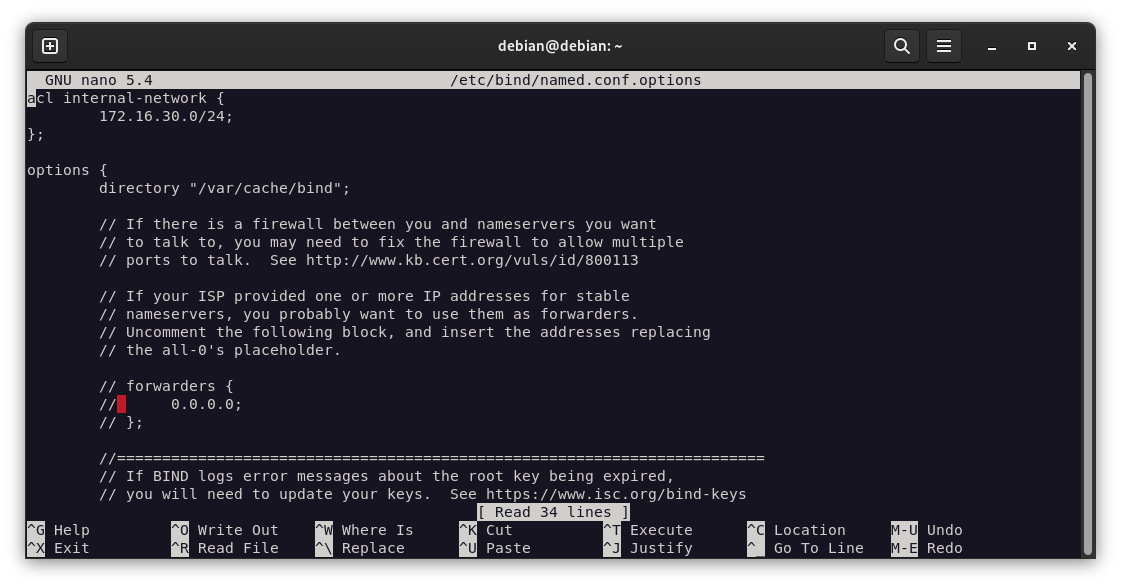
\includegraphics[scale=0.30]{02}
	\caption{Indicando el ACL para la zona interna.}
\end{figure}

Luego al final, indicamos las directivas que permiten las consultas al DNS con las ACL y un modo de consulta.

\begin{figure}[H]
	\centering
	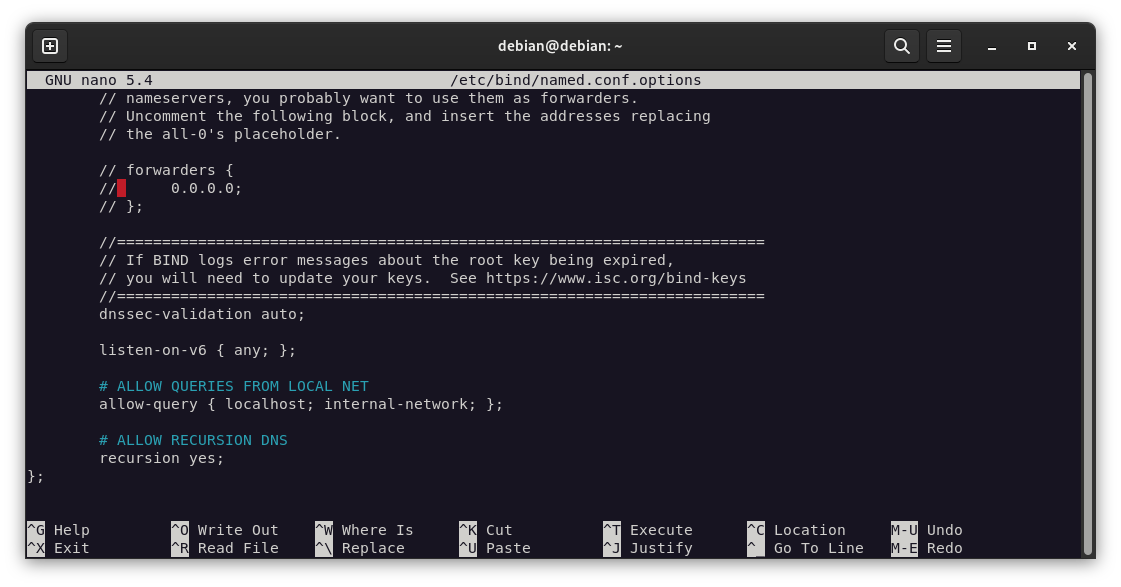
\includegraphics[scale=0.30]{03}
	\caption{Directivas para permitir las consultas.}
\end{figure}

\newpage
\section{Creando el fichero de configuración de las zonas internas}

Ahora debemos crear el fichero de configuración de la zona interna, indicado en \textbf{/etc/bind/named.conf}. Dicho fichero tiene dos subficheros, uno de la resolución normal de nombres y otro de la resolución inversa de nombres.

La resolución normal, consiste en que cuando le preguntas a tu DNS quién es pepe.com, este te busca si no tiene esa zona, desde la raíz primero el servidor DNS (root) ., luego el servidor autoritativo .com., luego el servidor DNS .com devuelve la IP de pepe.com.
\vspace{5mm}

En la resolución inversa, se apunta a un servidor de autoridad arpa., luego escala la petición a in-addr.arpa, luego va escalando en cada octeo de IPv4 hasta encontrar el DNS que esté en el nodo hoja que se corresponda con la IPv4 completa. En nuestro caso la IPv4 que se escribe como 172.16.30.0/24, se debe escribir al revés y sin la parte del host que se deja sin poner en el fichero de zona de resolución inversa. 

Cuando queramos buscar el nombre de dominio de un host, pero solo sabemos su dirección IP, tenemos que ponerla al revés de la siguiente manera, 10.30.16.172.in-addr.arpa, la cual crea una petición de resolución inversa.

Ahora creamos el fichero de la zona interna, la cual quedaría como en la siguiente captura. 

\begin{figure}[H]
	\centering
	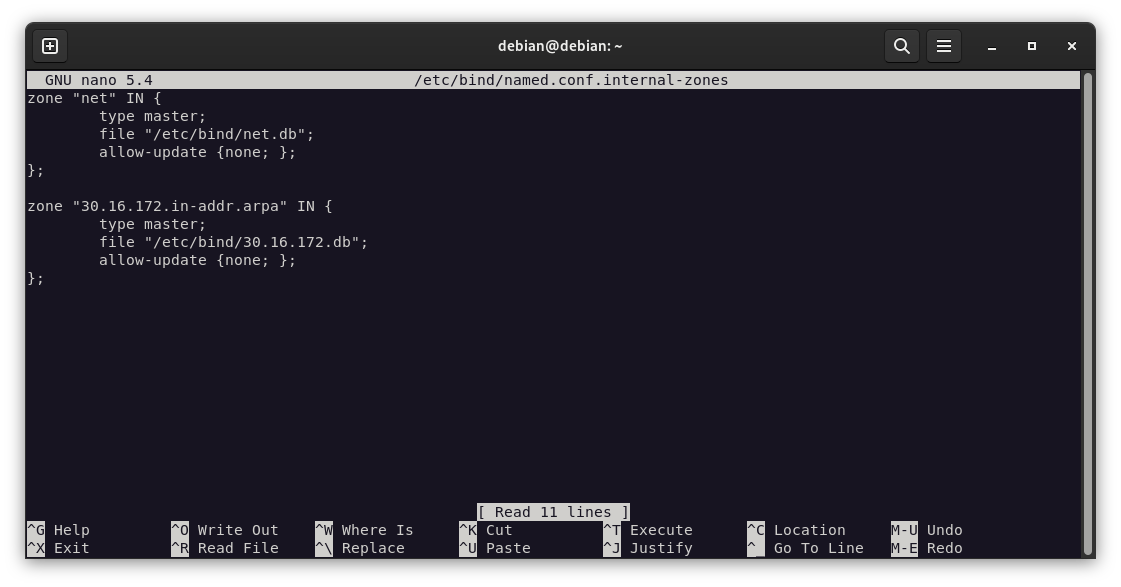
\includegraphics[scale=0.30]{04}
	\caption{Configuración del fichero de zonas.}
\end{figure}

En la captura podemos ver, que en cada zona hay un fichero asociado con una ruta absoluta, en dicho fichero, tenemos que generarlo con el de ejemplo que nos trae bind9 para evitar errores tipográficos. Para crear los ficheros hemos utilizado los siguientes comandos:

\begin{lstlisting}[style=mybash]
# Fichero DNS normal
sudo cp /etc/bind/db.empty /etc/bind/net.db
# Fichero DNS de Reverse resolution
sudo cp /etc/bind/db.0 /etc/bind/30.16.172.db
\end{lstlisting}

Primero configuramos la zona de resolución normal, esta zona tiene la característica de que aquí se alojan las resoluciones del tipo A, AAAA, NS, MX,...

\begin{figure}[H]
	\centering
	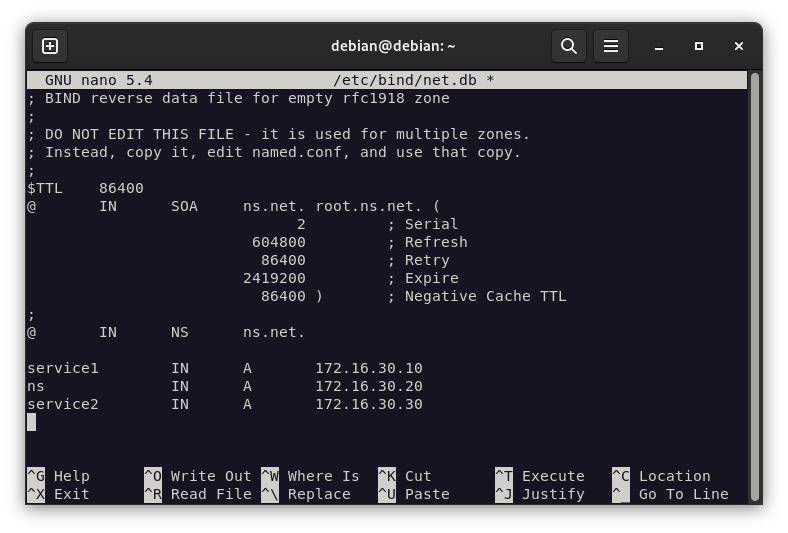
\includegraphics[scale=0.30]{05}
	\caption{Configuración de la zona .net.}
\end{figure}

Ahora configuramos la zona de resolución inversa, esta zona es la que tiene todos los PTR.

\begin{figure}[H]
	\centering
	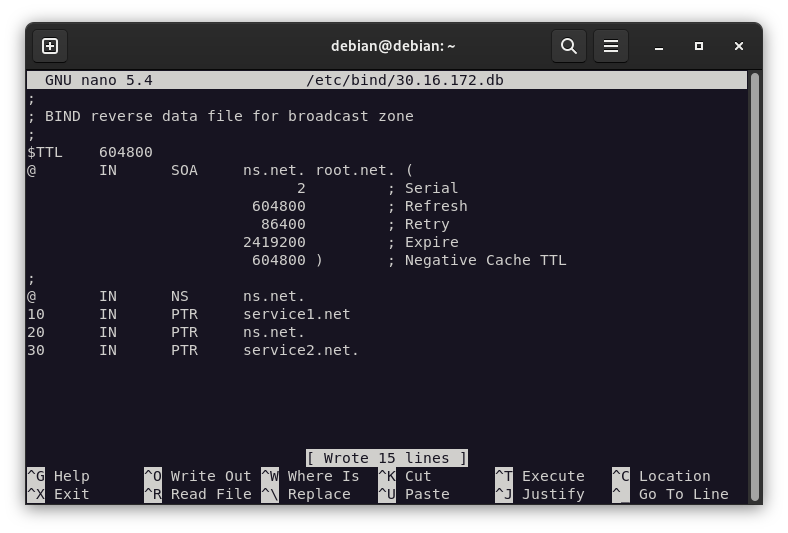
\includegraphics[scale=0.30]{06}
	\caption{Configuración de la zona inversa.}
\end{figure}

Una vez terminada la configuración de las zonas, tenemos que reiniciar el servicio bind9, el cual cuando consultamos el log, para que sepamos que el servicio está funcionando correctamente tenemos que tener las siguientes líneas de que se han cargado tanto nuestra zona, como las zonas que necesita el DNS.

\begin{lstlisting}[style=mybash]
sudo systemctl restart bind9.service
\end{lstlisting}

\begin{figure}[H]
	\centering
	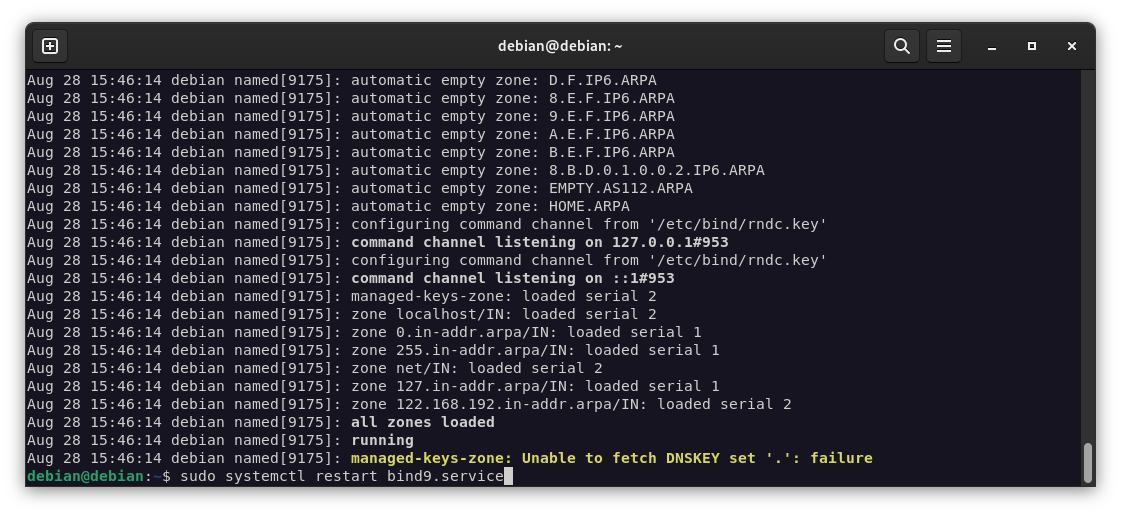
\includegraphics[scale=0.30]{07}
	\caption{Carga correcta del servicio bind9.}
\end{figure}

Una vez cargado el servicio DNS correctamente, tenemos que configurar en el fichero de configuración de las interfaces para poder indicar que el DNS es el propio y está en localhost.

\begin{figure}[H]
	\centering
	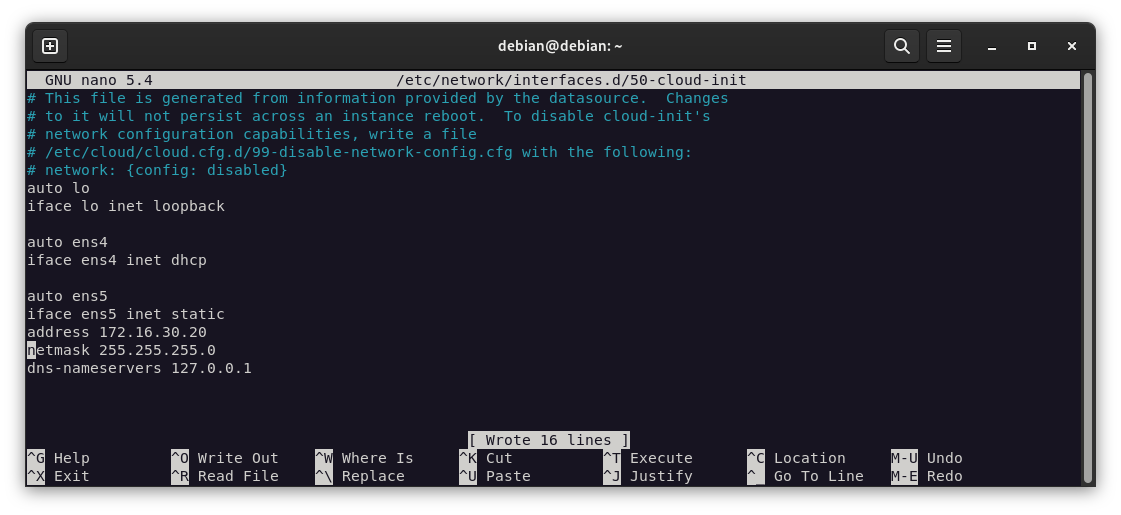
\includegraphics[scale=0.30]{08}
	\caption{Configuración de interfaces de red.}
\end{figure}

\newpage
\section{Pruebas con el DNS}

Se ha utilizado la herramienta de DIG para realizar las pruebas de la consulta de DNS.

\begin{figure}[H]
	\centering
	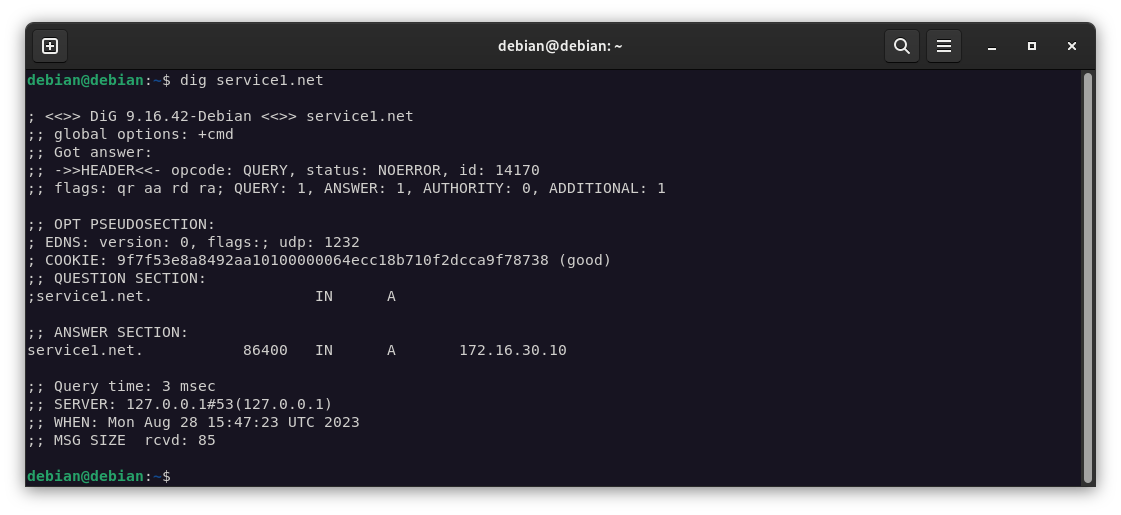
\includegraphics[scale=0.30]{09}
	\caption{Consulta de la IP del service1.net.}
\end{figure}

\begin{figure}[H]
	\centering
	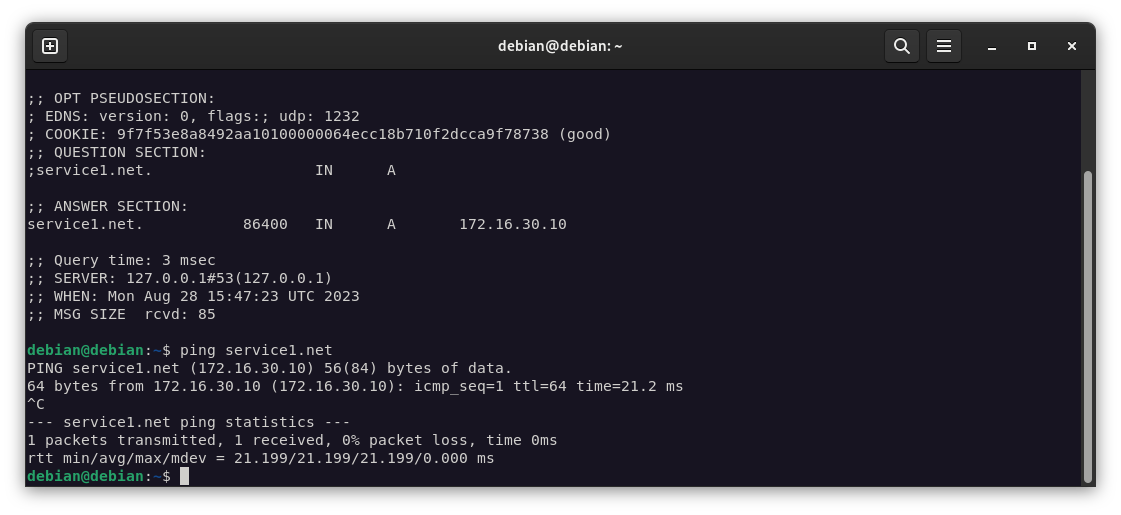
\includegraphics[scale=0.30]{10}
	\caption{Ping con resolución DNS a service1.net.}
\end{figure}

\begin{figure}[H]
	\centering
	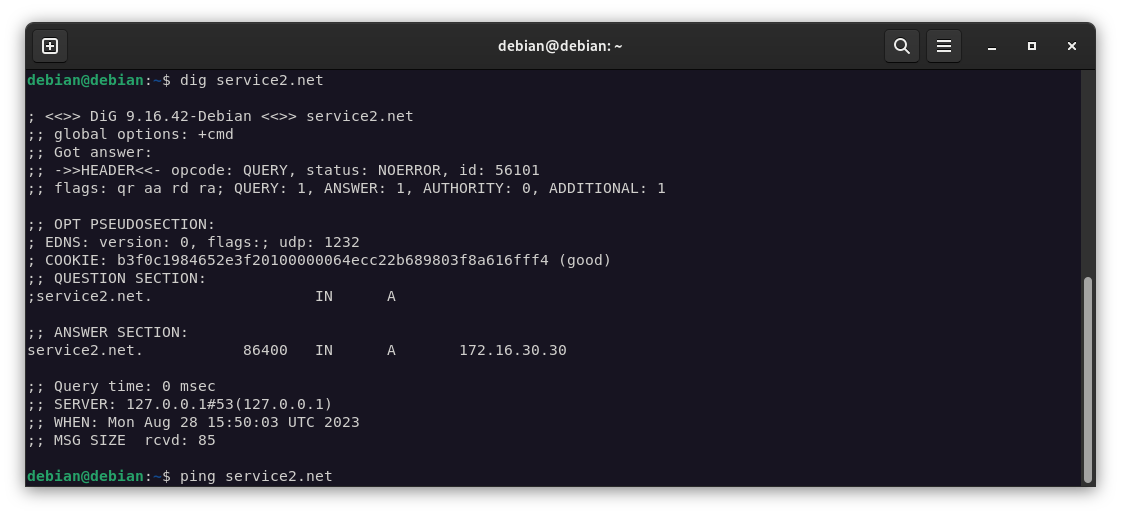
\includegraphics[scale=0.30]{11}
	\caption{Consulta de la IP del service2.net.}
\end{figure}

\begin{figure}[H]
	\centering
	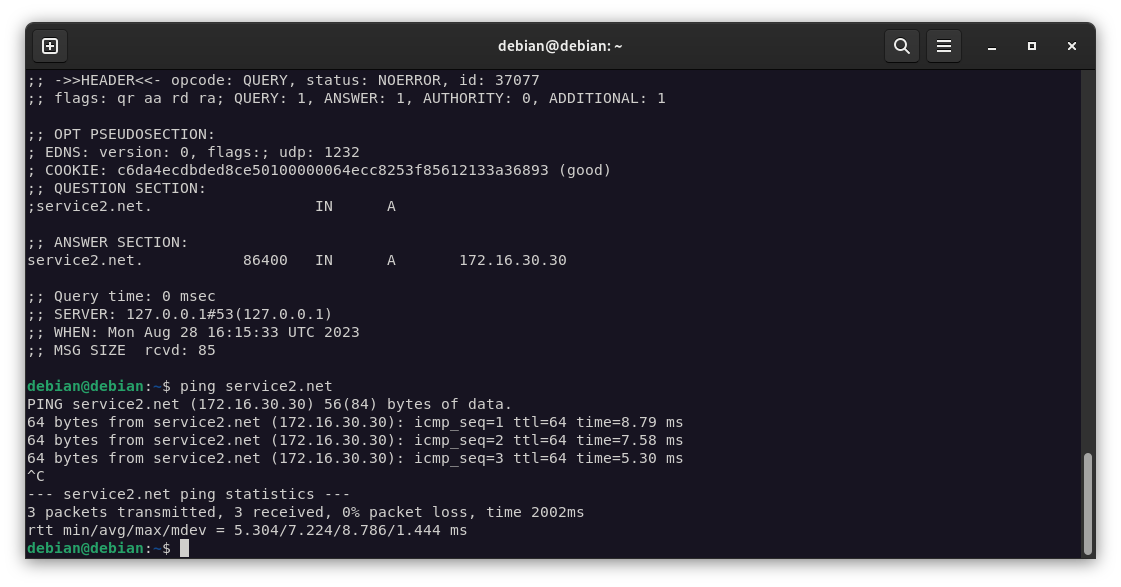
\includegraphics[scale=0.30]{12}
	\caption{Ping con resolución DNS a service2.net.}
\end{figure}

En el siguiente hacemos una consulta especial de DNS, donde indicamos que queremos saber quienes son los servidores DNS con el campo NS.

\begin{figure}[H]
	\centering
	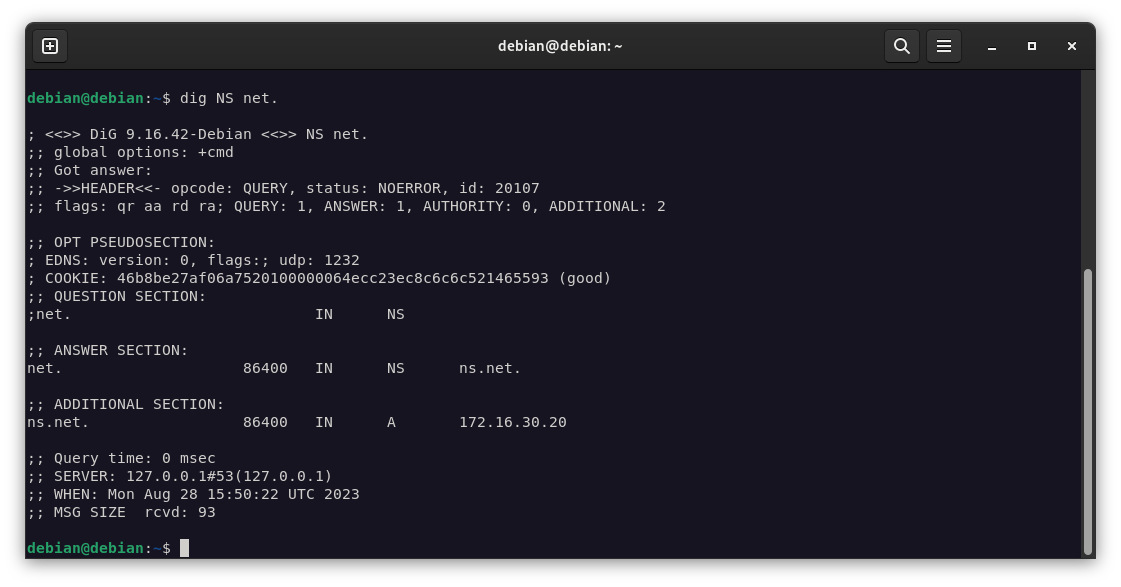
\includegraphics[scale=0.30]{13}
	\caption{Conociendo los servidores de nombres de autoridad en .net.}
\end{figure}

En la siguiente captura, hemos creado una consulta especial para obtener el registro PTR, para que el DNS nos devuelva el nombre completo de una dirección IP.

\begin{figure}[H]
	\centering
	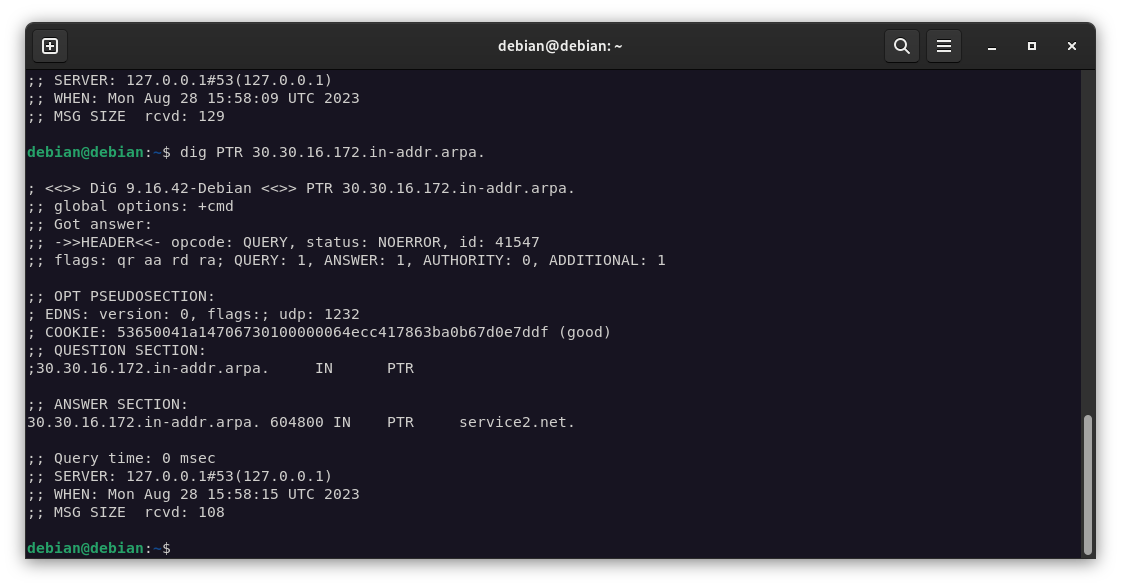
\includegraphics[scale=0.30]{14}
	\caption{Obteniendo el registro PTR de la ip 172.16.30.30 que nos devuelve el nombre servicio2.net.}
\end{figure}

Luego por último el comando dig permite la consulta sin tener que poner in-addr.arpa pasándole el parámetro -X para que te haga el nombre de resolución inversa.

\begin{figure}[H]
	\centering
	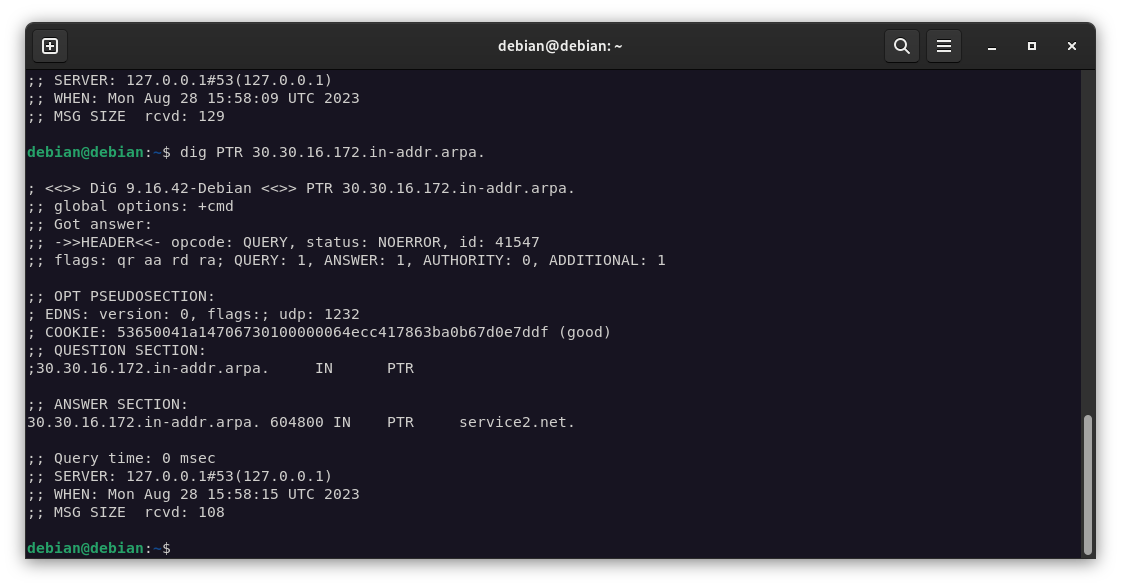
\includegraphics[scale=0.30]{14}
	\caption{Resolución inversa de 172.16.30.10.}
\end{figure}

% \vspace{5mm}


% \begin{lstlisting}[style=mybash]
%     # Para una base de datos concreta
%     mysqldump --user=tiendabd --password=password --databases tiendabd --add-drop-database --add-drop-table [--replace] --host=127.0.0.1 --result-file=dump.sql
% \end{lstlisting}



%\begin{figure}[H]
%	\centering
%	\includegraphics[scale=0.30]{cuestion_1_1}
%	\caption{Se puede ver que al no haber un fallo grave, el sistema lo nota como que sigue funcionando pero en un estado degradado.}
%\end{figure}

%\newpage

%Se pueden hacer include en latex
%\newpage

\section{Section}

\subsection{Subseccion}

\subsubsection{Subseccion}



%-------Bibliografia-----------------------------

%\newpage
\section{Bibliografía}

% Ejemplo
\footnote{Administración de mdadm - Por Red Hat}
\textcolor{blue}{\url{https://access.redhat.com/documentation/en-us/red_hat_enterprise_linux/8/html/managing_storage_devices/managing-raid_managing-storage-devices#monitoring-raid_managing-raid}}



\end{document}
